% IN55 - Particle System project report
% Spring 2014
% Authors : Adrien Berthet, Gautier Claisse and Karim Naaji

%----------------------------------------------------------------------------------------
%	PACKAGES AND DOCUMENT CONFIGURATIONS
%----------------------------------------------------------------------------------------

\documentclass[a4paper,10pt]{report}
\usepackage[margin=1.3in]{geometry}
\usepackage[utf8x]{inputenc}
\usepackage[T1]{fontenc}
\usepackage[french]{babel}
\usepackage{color,colortbl}
\usepackage{phdthesis}	% Much beautiful
\usepackage{fancyhdr}
\usepackage{graphicx}
\usepackage{hyphenat}	% Caesura

% Code Coloring with minted, use it as follow :
% \begin{figure}
%	\begin{minted}[bgcolor=bg,tabsize=4]{c}
%		printf("hello");
%	\end{minted}
% \end{figure}
\usepackage{minted}
\definecolor{bg}{rgb}{0.95,0.95,0.95}

\renewcommand*\rmdefault{phv} % Helvetica yeah yeah yeah

\setlength\parindent{0pt} % Removes all indentation from paragraphs

%----------------------------------------------------------------------------------------
%	DOCUMENT INFORMATION
%----------------------------------------------------------------------------------------

\title{Système de particules\\Projet d'IN55}
\author{Adrien \bsc{Berthet}, Gautier \bsc{Claisse} et Karim \bsc{Naaji}}
\date{\bsc{Printemps} 2014}

\begin{document}

\maketitle

%----------------------------------------------------------------------------------------
%	CONTENT
%----------------------------------------------------------------------------------------

% INTRODUCTION
\chapter*{Introduction}

Pour ce projet, le sujet abordant le système de particules (numéro 2) a été
retenu. Le choix de ce sujet s'est fait sur l'intérêt de la gestion physique de
ces particules de manière efficace. Dans les jeux vidéos, les systèmes de
particules sont trop peu souvent utilisés, pour gérer des phénomènes tels que la
fumée ou le feu, au profit de simples sprites (ce phénomène est toujours présent
même dans des jeux récents, à l'instar de Watch\_Dog).\\

\begin{center}
	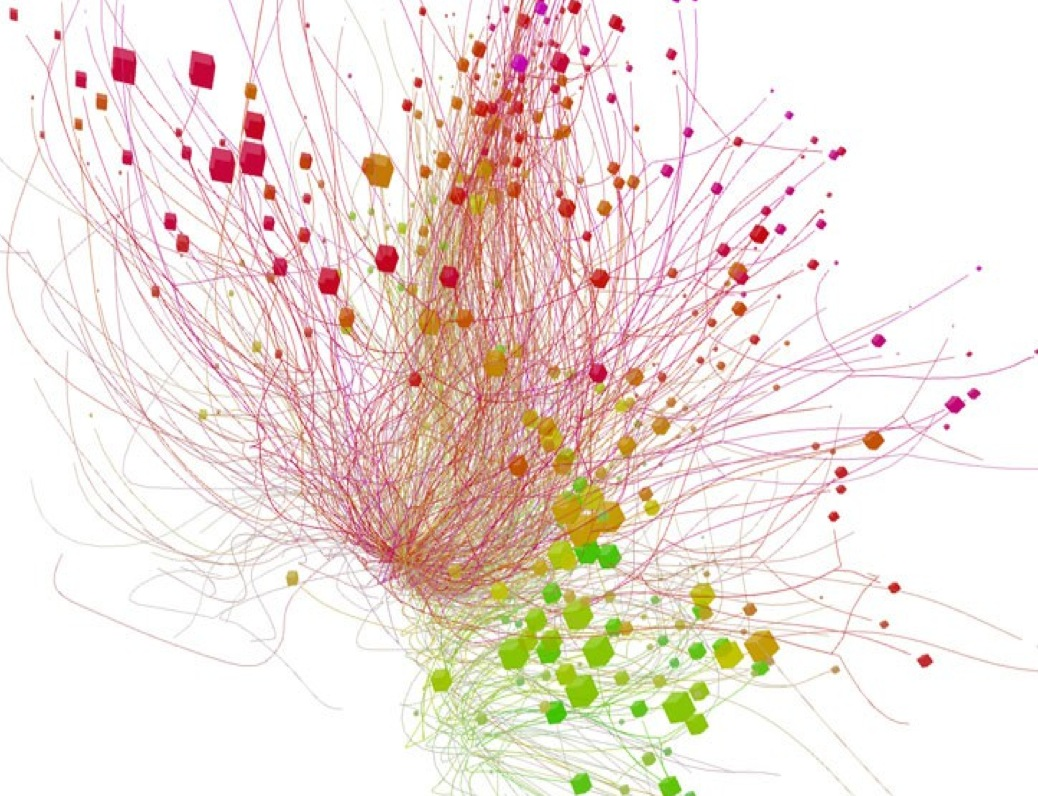
\includegraphics[width=0.7\textwidth]{img/01-introduction.jpg} 
\end{center}

Dans une première partie, le projet ainsi que les objectifs fixés seront
présentés. Les différentes phases de réalisation et d'implémentations de
l'application seront ensuite abordés. Ce rapport se terminera sur l'évocation
des problèmes rencontrés tout au long du projet, et les possibles améliorations
à apporter.

\addcontentsline{toc}{chapter}{Introduction}

% SUMMARY
\setcounter{tocdepth}{3}
\renewcommand{\contentsname}{Sommaire}
\tableofcontents

% PROJECT PRESENTATION
\chapter{Présentation du projet}

\section{Objectifs fixés}

Le sujet choisi avait pour consignes de paramétrer le rendu de particules
constitutives d'un phénomène physique (fumée, feu, eau) et de simuler leur
rendu dans une scène. La gestion de la physique doit être réalisée avec des
calculs GPU, c'est à dire avec GLSL et des shaders.\\

À partir de ces consignes, nous avons décidé de réaliser un programme de rendu
contenant un émetteur de particules. Cet objet sert de point d'émission aux
particules, qui vont alors se déplacer suivant différents \emph{patterns} précis
: par exemple un cône, une pyramide ou encore une sphère (émission non limitée 
dans tous les sens). Pour ne pas avoir d'attente trop haute, ces objectifs sont
les principaux fixés. D'autres, considérés comme secondaires, ont été évoqués.
Il serait ensuite possible de placer plusieurs émetteurs (directement par le 
code ou par l'utilisateur via la souris) et ainsi cela permettrait d'observer la
réaction de particules se rencontrant entre elles.\\

\section{Résultat final}

Le rendu final est celui escompté : deux types d'émissions sont disponibles
(émissions sphérique et cônique) et également un « plan » de particules qui a un
mouvement semblable à des vagues. L'ensemble des tranformations des particules a
été réalisée à travers un ensemble de \emph{shaders}, que cela soit pour les
mouvements comme pour les couleurs. L'interface est également présente, même si
limitée, par manque de temps principalement et peu de connaissance sur le sujet
des widgets Qt (voir paragraphe \ref{gui}).

% We need screen cap here pls
\begin{figure}[h]
	\begin{center}
		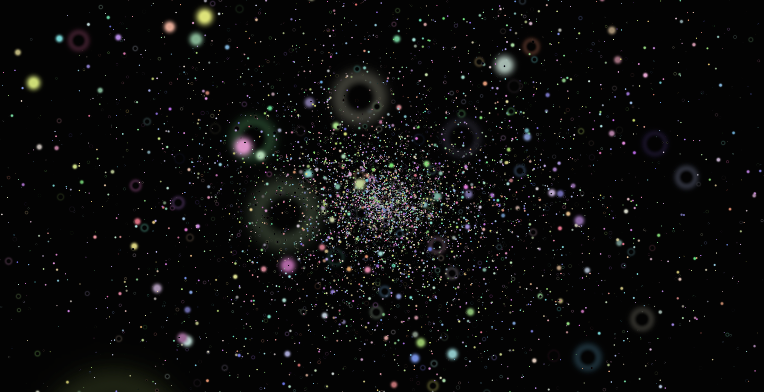
\includegraphics[width=0.7\textwidth]{img/21-sphere.png}
	\end{center}
	\caption{Rendu à émission spérique}
\end{figure}

\begin{figure}[h]
	\begin{center}
		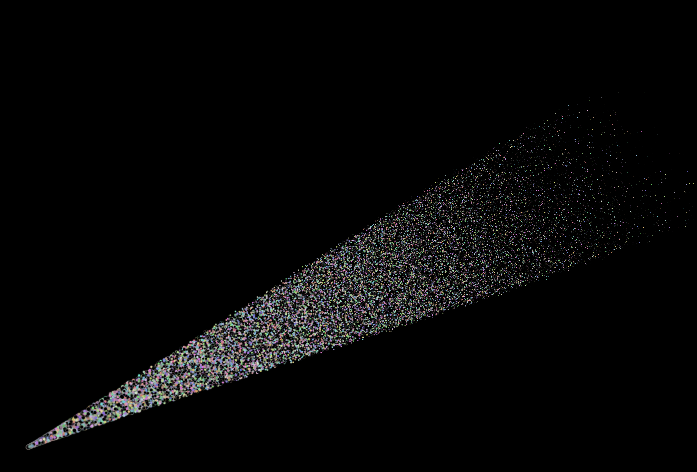
\includegraphics[width=0.8\textwidth]{img/22-cone.png}
	\end{center}
	\caption{Rendu avec diffusion cônique}
\end{figure}

\begin{figure}[h]
	\begin{center}
		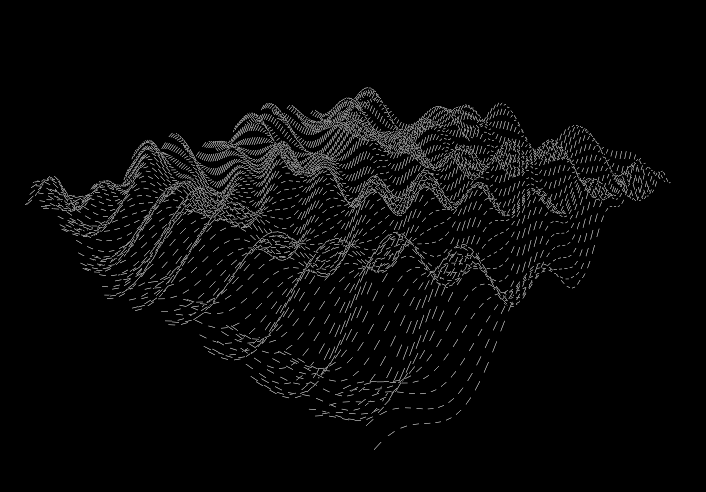
\includegraphics[width=0.8\textwidth]{img/23-waves.png}
	\end{center}
	\caption{Rendu avec des vagues}
\end{figure}


% MODELISATION / IMPLEMENTATION
\chapter{Modélisation et implémentation}

\section{Fonctionnement global}

Résumé simplement, on peut dire qu'il y a création d'une scène dans
laquelle on met des noeuds. Ces noeuds correspondent à des objets qui seront contenus
dans la scène. Comme dit précédemment, nous avons deux types finaux pour les noeuds:
l'\emph{EmitterNode} et le \emph{WaveParticleNode}. \\

Les deux ont un comportement identique. Ils vont créer des vertex et leur donner des
attributs initiaux. Ces attributs peuvent être une position, une vitesse, une couleur
ou encore un temps de vie par exemple. Lorsque les vertex sont initialisés, le noeud ne
va plus réellement s'occuper d'eux. En effet, ils sont ensuite gérés uniquement par des
shaders. Tous les traitements ultérieurs subis par les vertex sont effectués par des 
shaders. Les actions à exercer sur ces vertex sont calculées à partir des attributs initiaux
de chaque vertex et du temps. L'exemple le plus visuel est la position. Ainsi,
il n'est par exemple pas possible de gérer les collisions entre particules mais c'est le GPU qui gère
tous ces calculs.\\

L'introduction du \emph{ShaderManager} a été très utile. C'est l'objet qui va gérer tous les
shaders utilisés dans le projet.\\

L'initialisation de ces attributs est simplifiée par l'introduction de \emph{Samplers}.
Ces \emph{Samplers} servent uniquement à générer des données de manière aléatoire. Par exemple
le \emph{ConeSampler} va simplement générer des vecteurs de directions (partant de la base du cône
en prenant en compte son ouverture).

\begin{figure}[h]
	\begin{center}
		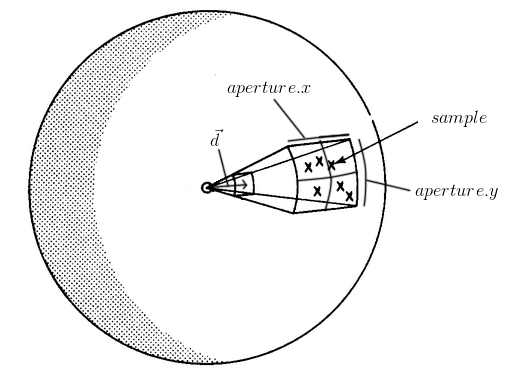
\includegraphics[width=0.5\textwidth]{img/conesampler.png}
	\end{center}
	\caption{Shéma du \emph{ConeSampler}}
\end{figure}

L'introduction du \emph{ShaderManager} a été très utile. C'est l'objet qui va gérer tous les
shaders utilisés dans le projet.

\section{Diagramme de classe}

Pour posséder une cohérence dès le début et tout au long du projet, un diagramme
de classe a été crée.

\begin{figure}[h]
	\begin{center}
		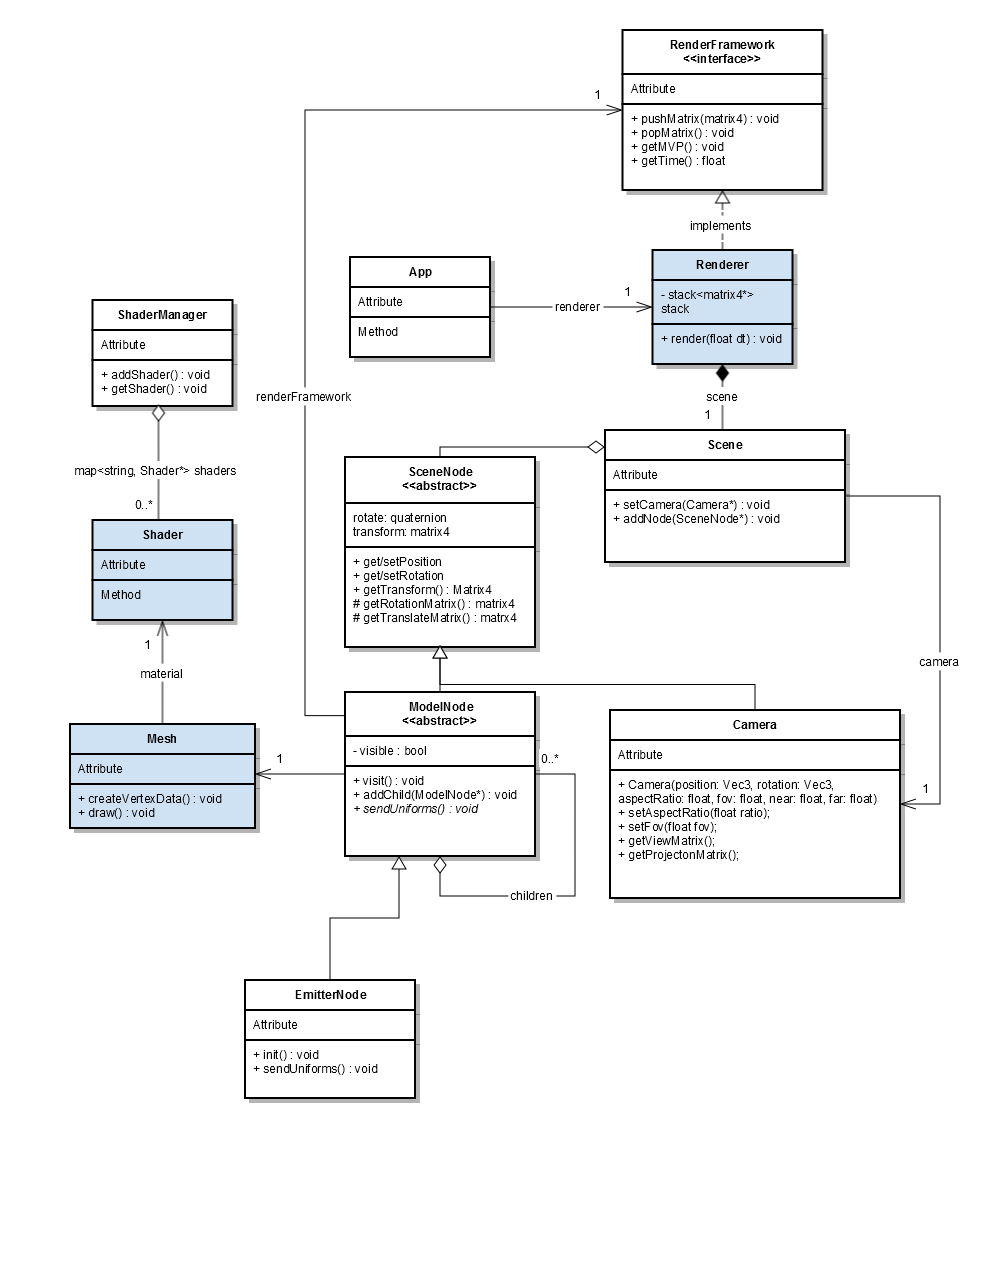
\includegraphics[width=0.9\textwidth]{img/UML.png}
	\end{center}
	\caption{Diagramme UML du projet}
\end{figure}

\newpage

\section{Structure de données}

Comme évoqué précédemment, toute la partie physique des particules est gérée via
des shaders. Ceux-ci récupèrent plusieurs données dans le buffer. Chaque
élément de ces données va représenter un attribut d'une particule. Ainsi,
celles-ci sont définies par une position, une couleur, une vitesse, un
\emph{timer} de vie et une durée de vie. Ces cinq attributs sont présents dans
les shaders, et une \emph{struct} est existante dans la classe
\emph{EmitterNode}.

\begin{figure}[h]
	\begin{minted}[bgcolor=bg]{c}
struct EmitterVertexData {
    Vec3 position;
    Color color;
    Vec3 velocity;
    float delay;
    float lifetime;
};
	\end{minted}
	\caption{Structure \emph{EmitterVertexData}}
\end{figure}



% PROBLEMS / DIFFICULTIES
\chapter{Difficultés rencontrées}

Un certain nombre de problèmes ont été rencontrés tout au long du développement
du projet. Ces complications sont de nature technique (par exemple avec la mise
en place du GUI, la gestion de l'alpha avec les textures) mais principalement de
nature géométrique.

\section{Notations matricielles américaine et française}

Le premier problème, qui a apporté un certain sentiment de confusion, a été le
sens de notation. En effet, les notations américaine et française pour
l'écriture matricielle ne sont pas les mêmes. Les colonnes et les lignes sont
inversées entre les deux.\\

Comme il a été décidé de ne pas reprendre le framework fourni dans les TPs, mais
de réécrire complétement une plateforme from scratch, tous les calculs pour des 
classes de base (\emph{Matrix4}, \emph{Vec3}, etc...) ont été réalisés en utilisant la
notation matricielle française. Cependant, le système de la caméra libre a été
conçu d'après le TP concerné et plusieurs ressources sur Internet. Il y a donc
eu une confusion sur l'écriture, puisque la totalité des ressources consultées 
concernaient la notation américaine. Ainsi, une quantité importante de soucis
liés à ces malentendus est apparue, principalement pour la gestion des
transformations de la camera, et le calcul de la matrice \emph{MVP}. Par exemple, une
déformation importante de l'objet était présente, comme sur une caméra avec un
objectif de type FishEye. Mais le but étant d'obtenir une caméra classique,
l'ensemble des matrices a été uniformisé dans la notation française.

\section{Rotation semi-automatique de la caméra}

La gestion de la caméra est sans doute l'élément le plus difficile de ce projet.
Celle ci est contrôlée avec les touches fléchées, mais également avec la souris
(il faut appuyer sur la touche \emph{Alt} pour verrouiller/déverrouiller le
mouvement de la souris). Lorsque l'on effectue plusieurs rotations avec la
souris, alors que celle-ci est censée effectuer un simple mouvement sur deux
axes (x et y), il semblerait qu'elle réalise également une rotation sur l'axe z.
Ce problème est apparu et a disparu à plusieurs reprises, sans que la véritable
raison soit réellement identifiée.

\section{Gestion de l'alpha des textures}

Les particules sont toutes considérées comme un point unique de l'espace, sur
lesquelles est appliquée une texture. Dans un premier temps, la texture était un
simple carré blanc. Puis celle-ci a évolué pour une image plus complexe,
comportant un canal alpha.
\newpage

\begin{figure}[h]
	\begin{center}
		
\includegraphics[width=0.2\textwidth]{img/33-texture.png}
	\end{center}
	\caption{Texture avec présence du canal alpha}
\end{figure}

Par défaut, OpenGL ne reconnaît aucun canal alpha avec les textures. Il faut le
préciser à l'aide des constantes spécifiques. Le chargement de la texture se
fait à travers la classe \emph{Texture}. Dans un premier temps, il a été convenu
d'utiliser la fonction \emph{glBlendFunc} avec différentes constantes, comme
\emph{GL\_SRC\_ALPHA}. Cependant cette fonction n'a pas convenu à l'usage ci-présent,
car elle d'une part beaucoup plus utilisée pour la gestion des couleurs
directement en OpenGL, et d'autre part la texture n'est pas appliquée sur une 
zone spécifique, mais sur un point.\\

C'est dans la fonction \emph{glTexImage2D} qu'il faut s'orienter. Celle-ci possède
notamment un paramètre permettant de définir le nombre de couleurs composant
l'image à utiliser en texture. La constante \emph{GL\_RGBA} est à associer à cette
fonction, et permet ainsi un gestion du canal alpha pour cette texture de
particule.

\section{Insertion du rendu OpenGL dans un GUI}\label{gui}

Une des consignes du projet était d'avoir une interface Qt autour de la fenêtre
de rendu OpenGL. Cette interface doit permettre, au travers de boutons ou autres
éléments d'interface, de changer plusieurs paramètres de l'émetteur mis en
place. Personne ne possédant d'expérience avec les GUI et Widget Qt, un
apprentissage en plus a dû être réalisé. Dans un premier temps, une fenêtre Qt 
de type « MainWindow » a été utilisé. Pour des raisons qui sont toujours
obscures (il s'agirait sans doute d'un problème lié à la plateforme Mac OSX), il
est impossible de dessiner le rendu OpenGL. Un message indique que la taille du
widget contenant le rendu est trop petite, même pour une taille dix fois plus
grande que le rendu.\\

La solution est d'avoir une base simple, c'est à dire un simple Widget Qt en
fenêtre principale. Il suffit d'adapter par la suite l'application existante
pour l'inclure dans ce nouveau widget, puis de réaliser les \emph{bind}
nécessaires pour relier les actions des boutons de l'interface aux actions de
l'application. Il ne faut également pas oublier de déplacer la prise en compte
des évènements claviers dans le widget parent, mais pas nécessairement les
évènements souris.


% POSSIBLE IMPROVEMENTS
\chapter{Améliorations possibles}

% TODO Lunpe
% Ajout de trajectoires différentes, gestion de plusieurs points d'émission,
% intégration à un environnement, flexibilité

Bien qu'on puisse considérer le projet comme fini, il y a toujours des choses
que nous pourrions ajouter ou améliorer. Ce sont des améliorations qui sont
dans le domaine du nice-to-have et que nous n'avons pas implémenté.

\section{Ajout de trajectoires différentes}
Nous avons une base de shaders très simples qui permettent de déplacer nos
particules correctement. Cela dit, ces déplacements ne sont pas toujours très
impressionnants. Une amélioration possible serait d'ajouter plein de types de
forces différentes et de sélectionner lesquelles appliquer à nos particules
(gravité, force radiale, rappel vers le point d'émission, ajout d'un spin à la
trajectoire ou autres). Certaines de ces choses seraient faciles à implémenter (gravité
ou rappel vers le point d'émission) alors que d'autres demanderaient plus de réflexion
afin de déterminer les bonne forces (et dans quelles directions) appliquer uniquement
en fonction du temps. Il serait ainsi possible de conjuguer toutes ces forces
afin d'avoir des comportements plus poussés.

\section{Gestion de plusieurs points d'émission}
Actuellement, la scène ne comporte qu'un noeud de particules. Augmenter ce
nombre pourrait être intéressant autant d'un point de vue visuel qu'utilitaire.
En effet, monter un système de particules possédant plusieurs sources ou types
de particules permet de faire des choses bien plus aguichantes qu'un simple émetteur
de particules. La raison pour laquelle nous n'avons pas implémenté cette fonction est
que, derrière ses airs triviaux, elle nous pose un problème dans la gestion des shaders.
En effet, créer un noeud deux fois recquiert d'utiliser le shader deux fois, et en faisant
cela on crée le même shader plusieurs fois ce qui n'est pas possible dans notre cas.

\section{Intégration à un environnement}
La dernière amélioration notoire que nous avons pensé faire est d'intégrer nos systèmes
de particules dans un environnement comportant d'autre objets 3D. On pourrait donner
en exemple le fait d'avoir un modèle de torche et de placer un émetteur de particules
ayant des textures se rapprochant de la fumée afin d'avoir l'impression que la torche fume.
Cependant, il serait aussi possible de faire une intégration à un environnement bien plus poussée.
En effet, en passant des objets 3D simples au vertex shader, il serait possible de faire
intéragir nos particules et ces objets: des balles qui rebondissent au sol par exemple. 


% CONCLUSION
\chapter*{Conclusion}
Ce projet nous a permis de bien mettre en pratique certains des concepts que
nous avons abordé pendant les cours d'IN55. Il nous a permis de bien
comprendre les aspects que nous y avons abordé et nous sommes tous
satisfaits du résultat. En effet, bien que certains aspects puissent encore être
améliorés, la plupart objectifs que nous nous étions fixés sont atteints.

\addcontentsline{toc}{chapter}{Conclusion}

\end{document}
